\section{Fast FullSubNet}
\label{sec:fast-fullsubnet}
Subband approaches have been widely used in speech enhancement tasks, as they allow the model to focus on local spectral patterns.
Many variants of the subband approach have been proposed, focusing on improving the model's ability in noise reduction and speech enhancement.
However, these approaches often suffer from high computational complexity and slow inference speed.
To address this issue, Hao and Li\cite{hao2023fast} proposed a novel, lightweight framework called Fast FullSubNet.
Fast FullSubNet is a subband-based speech enhancement model that is designed to be fast and efficient while maintaining high performance in noise reduction tasks.
It utilizes the mel-frequency domain to reduce the number of frequency bands while maintaining the spectral information.
The Mel-frequency representation effectively condenses speech spectra while concurrently maintaining spectral information crucial for human auditory perception.

\subsection{Model Architecture}
The Fast FullSubNet model consists of three main components: Full-band model $F_{l2m}$ (encoder),
Sub-band model $S$ (bottleneck) and Full-band model $F_{m2l}$ (decoder). Figure \ref{fig:fast-fullsubnet} illustrates the architecture of Fast FullSubNet.

\begin{figure}[H]
    \centering
    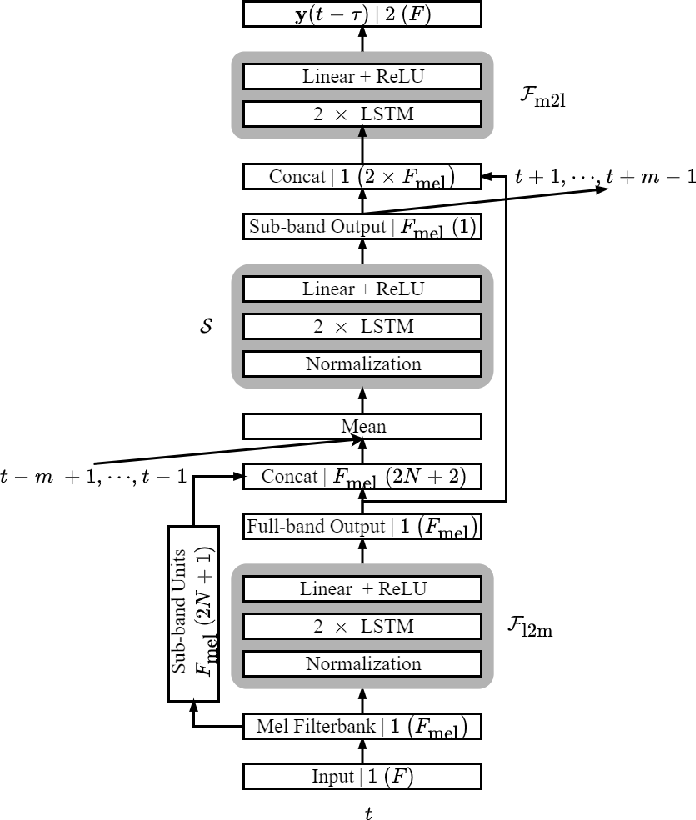
\includegraphics[width=0.8\textwidth]{images/related_work/ffsn/arch.png}
    \caption{Diagram of Fast FullSubNet. The right parts of rectangle boxes
        show feature dimensions, e.g., “1 (F)” represents a F-dimension vector.
        “Fmel(2N + 2)” denotes Fmel independent (2N + 1)-dimensional vectors.}
    \label{fig:fast-fullsubnet}
\end{figure}

\subsubsection{Encoder}
The mel-scale spectral magnitude undergoes initial processing by the full-band model, Fl2m, which extracts global spectral characteristics
and long-range dependencies across bands. Specifically, the linear frequency signal \( x(t, f) \) is transformed into the mel-frequency domain
as \( x_{\text{mel}}(t, f) \), where \( f \in [0, \ldots, F_{\text{mel}} - 1] \)
and \( F_{\text{mel}} \) denotes the number of mel frequencies.
The input vector to Fl2m at time \( t \) is represented as
\[ x(t) = [x_{\text{mel}}(t, 0), \ldots, x_{\text{mel}}(t, F_{\text{mel}} - 1)]^T \in \mathbb{R}^{F_{\text{mel}}} \]
This feature vector sequence is then processed by two layers of LSTM. The full-band model produces a spectral embedding of the same dimension as \( x(t) \),
with each mel-frequency corresponding to one hidden unit. This spectral embedding complements the subsequent sub-band model by providing additional informative features.

\subsubsection{Bottleneck}
The sub-band model operates on mel-frequencies independently within a shared network structure. It predicts clear speech by leveraging
the stationary nature of signals and the local spectral patterns specific to speech. Each input to the sub-band model incorporates two main sources.
Firstly, for a given frequency \( f \), the input consists of the noisy mel-spectra at that frequency and \( N \) adjacent frequencies on each side.
Secondly, it includes the output of the full-band model at frequency \( f \), denoted as \( \text{Fl2m}(x(t))(f) \). These sources are concatenated
to form the input vector
\begin{equation}
    \label{eq:fast-fullsubnet-input}
    x_{\text{sub}}(t, f) = [x_{\text{mel}}(t, f - N), \ldots, x_{\text{mel}}(t, f + N), \text{Fl2m}(x(t))(f)]^T \in \mathbb{R}^{2N+2}
\end{equation}

% \[ x_{\text{sub}}(t, f) = [x_{\text{mel}}(t, f - N), \ldots, x_{\text{mel}}(t, f + N), \text{Fl2m}(x(t))(f)]^T \in \mathbb{R}^{2N+2} \]
This feature vector sequence is uniformly processed using two LSTM layers across all frequencies. Each mel-frequency processed by the sub-band model yields a
single-dimensional hidden unit output.
To accelerate inference speed, the feature sequence is downsampled by a factor of \( m \) before being processed by the bottleneck, exploiting redundancies among
successive samples.

\subsubsection{Decoder}
The full-band model Fm2l reverses the mel-frequency transformation to obtain linear-frequency representations. It combines the outputs of the full-band model Fl2m and the sub-band Model S into a concatenated input vector xm2l(t) for Fm2l:
\begin{equation}
    \label{eq:fast-fullsubnet-m2l}
    x_{m2l}(t) = [Fl2m(x(t))^T, S(x_{\text{sub}}(t, 0)), \ldots, S(x_{\text{sub}}(t, F_{\text{mel}} - 1))]^T \in \mathbb{R}^{2F_{\text{mel}}}
\end{equation}
% \[ x_{m2l}(t) = [Fl2m(x(t))^T, S(x_{\text{sub}}(t, 0)), \ldots, S(x_{\text{sub}}(t, F_{\text{mel}} - 1))]^T \in \mathbb{R}^{2F_{\text{mel}}} \]
This input is processed by two layers of LSTM followed by a linear layer to predict the final linear-frequency output. The model aims to predict the real-valued complex-valued Ideal Ratio Mask (cIRM) y(t) for each time-frequency bin:
\begin{equation}
    \label{eq:fast-fullsubnet-output}
    y(t) = [R\{y(t, 0)\}, I\{y(t, 0)\}, \ldots, R\{y(t, F - 1)\}, I\{y(t, F - 1)\}]^T \in \mathbb{R}^{2F}
\end{equation}
Here, R{} and I{} denote the real and imaginary parts of the complex number, respectively. This mel-to-linear model functions similarly to neural vocoders used in Text-to-Speech (TTS) applications, converting mel-frequency
representations to linear-frequency representations, with the capability to enhance speech using noisy signal phases.

\subsection{Experimental Setup}
\subsubsection{Dataset}
To ensure a fair comparison with FullSubNet, experiments were conducted on the DNS challenge dataset \cite{reddy2020} from INTERSPEECH 2020.
The training involved synthesizing noisy-clean speech pairs using dynamic mixing strategies similar to FullSubNet. Before each epoch, 75\%
of clean speech clips were mixed with room impulse responses from two databases, and combined with noise at varying SNR levels (-5 dB to 20 dB).
Training over ten epochs exposed the model to over 5000 hours of data. The evaluation used the DNS Challenge test dataset, consisting of 150 noisy clips each with and without reverberation,
and SNRs ranging from 0 dB to 20 dB.

\subsubsection{Training}
The audio signals are sampled at 16000 Hz, and their Short-Time Fourier Transform (STFT) uses a 32 ms (512 samples) Hanning window with a 16 ms hop size.
Mel-frequency analysis employs 64 bins. Training utilizes the Adam optimizer with a learning rate of 0.001, and to maintain consistency with prior work,
a two-frame output delay (equating to 32 ms) is implemented to allow the model to utilize future information effectively.
The training sequence length is set at T = 192 frames (about 3 seconds). Mean Squared Error (MSE) is employed as the loss function throughout the study.


\subsection{Conclusion}
Fast FullSubNet is a lightweight, efficient subband-based speech enhancement model that maintains high performance in noise reduction tasks.
The model utilizes the mel-frequency domain to reduce the number of frequency bands while preserving spectral information.
The Fast FullSubNet model consists of three main components: Full-band model $F_{l2m}$ (encoder), Sub-band model $S$ (bottleneck), and Full-band model $F_{m2l}$ (decoder).
The model was trained on the DNS Challenge dataset from INTERSPEECH 2020, and evaluation was conducted on the DNS Challenge test dataset.